\section{Background}
\label{sec:overview}

We review the background in stateless model checking and data-race analysis using the example program in Figure~\ref{fig:example}.

\subsection{Stateless Model Checking}

Stateless model checking \cite{verisoft} is a testing technique for systematically exploring the possible thread interleavings of a concurrent program.
A stateless model checker executes the program repeatedly, each time according to a new thread interleaving, until the state space (or the CPU budget) is exhausted.
Rather than identifying suspicious conditions which may include false alarms, the approach of many static analyses \cite{racerx,coverity},
stateless model checkers focus on concrete observed failures such as assertions, deadlocks, and segfaults.

\begin{figure}[t]
	\small
\begin{tabular}{rll}
	& \multicolumn{2}{c}{\texttt{int x = 0; mutex\_t mx;}} \\
	& {\bf Thread 1} & {\bf Thread 2} \\
	1 & \texttt{\hilight{orange}{mutex\_lock(\&mx);}} & \\
	2 & \texttt{int tmp = x;} &\\
	3 & & \texttt{atomic\_xadd(\&x, 1);} \\
	4 & & \texttt{\hilight{olivegreen}{yield();}} \\
	5 & & \texttt{atomic\_xadd(\&x, 1);} \\
	6 & \texttt{x = tmp + 1;} & \\
	7 & \texttt{\hilight{commentblue}{mutex\_unlock(\&mx);}} & \\
	8 & & \texttt{assert(x >= 2);} \\
	%1 & \texttt{\hilight{brickred}{x->foo = ...;}} & \\
	%2 & \texttt{\hilight{olivegreen}{free}(x);} \\
	%3 & & \texttt{\hilight{commentblue}{// x's memory recycled}} \\
	%4 & & \texttt{y~=~\hilight{olivegreen}{malloc}(sizeof *y);} \\
	%5 & & \texttt{\hilight{commentblue}{// ...initialize...}}\\
	%6 & & \texttt{publish(y);} \\
	%7 & & \texttt{\hilight{brickred}{y->bar = ...;}} \\
\end{tabular}
\caption{Example program with a data-race bug. In this interleaving, the assertion on line 8 will fail. Two data-race preemptions are required to expose the bug: one just before thread 1's line 6, and one just before thread 2's line 8.}
\label{fig:example}
\end{figure}

\begin{figure}[t]
	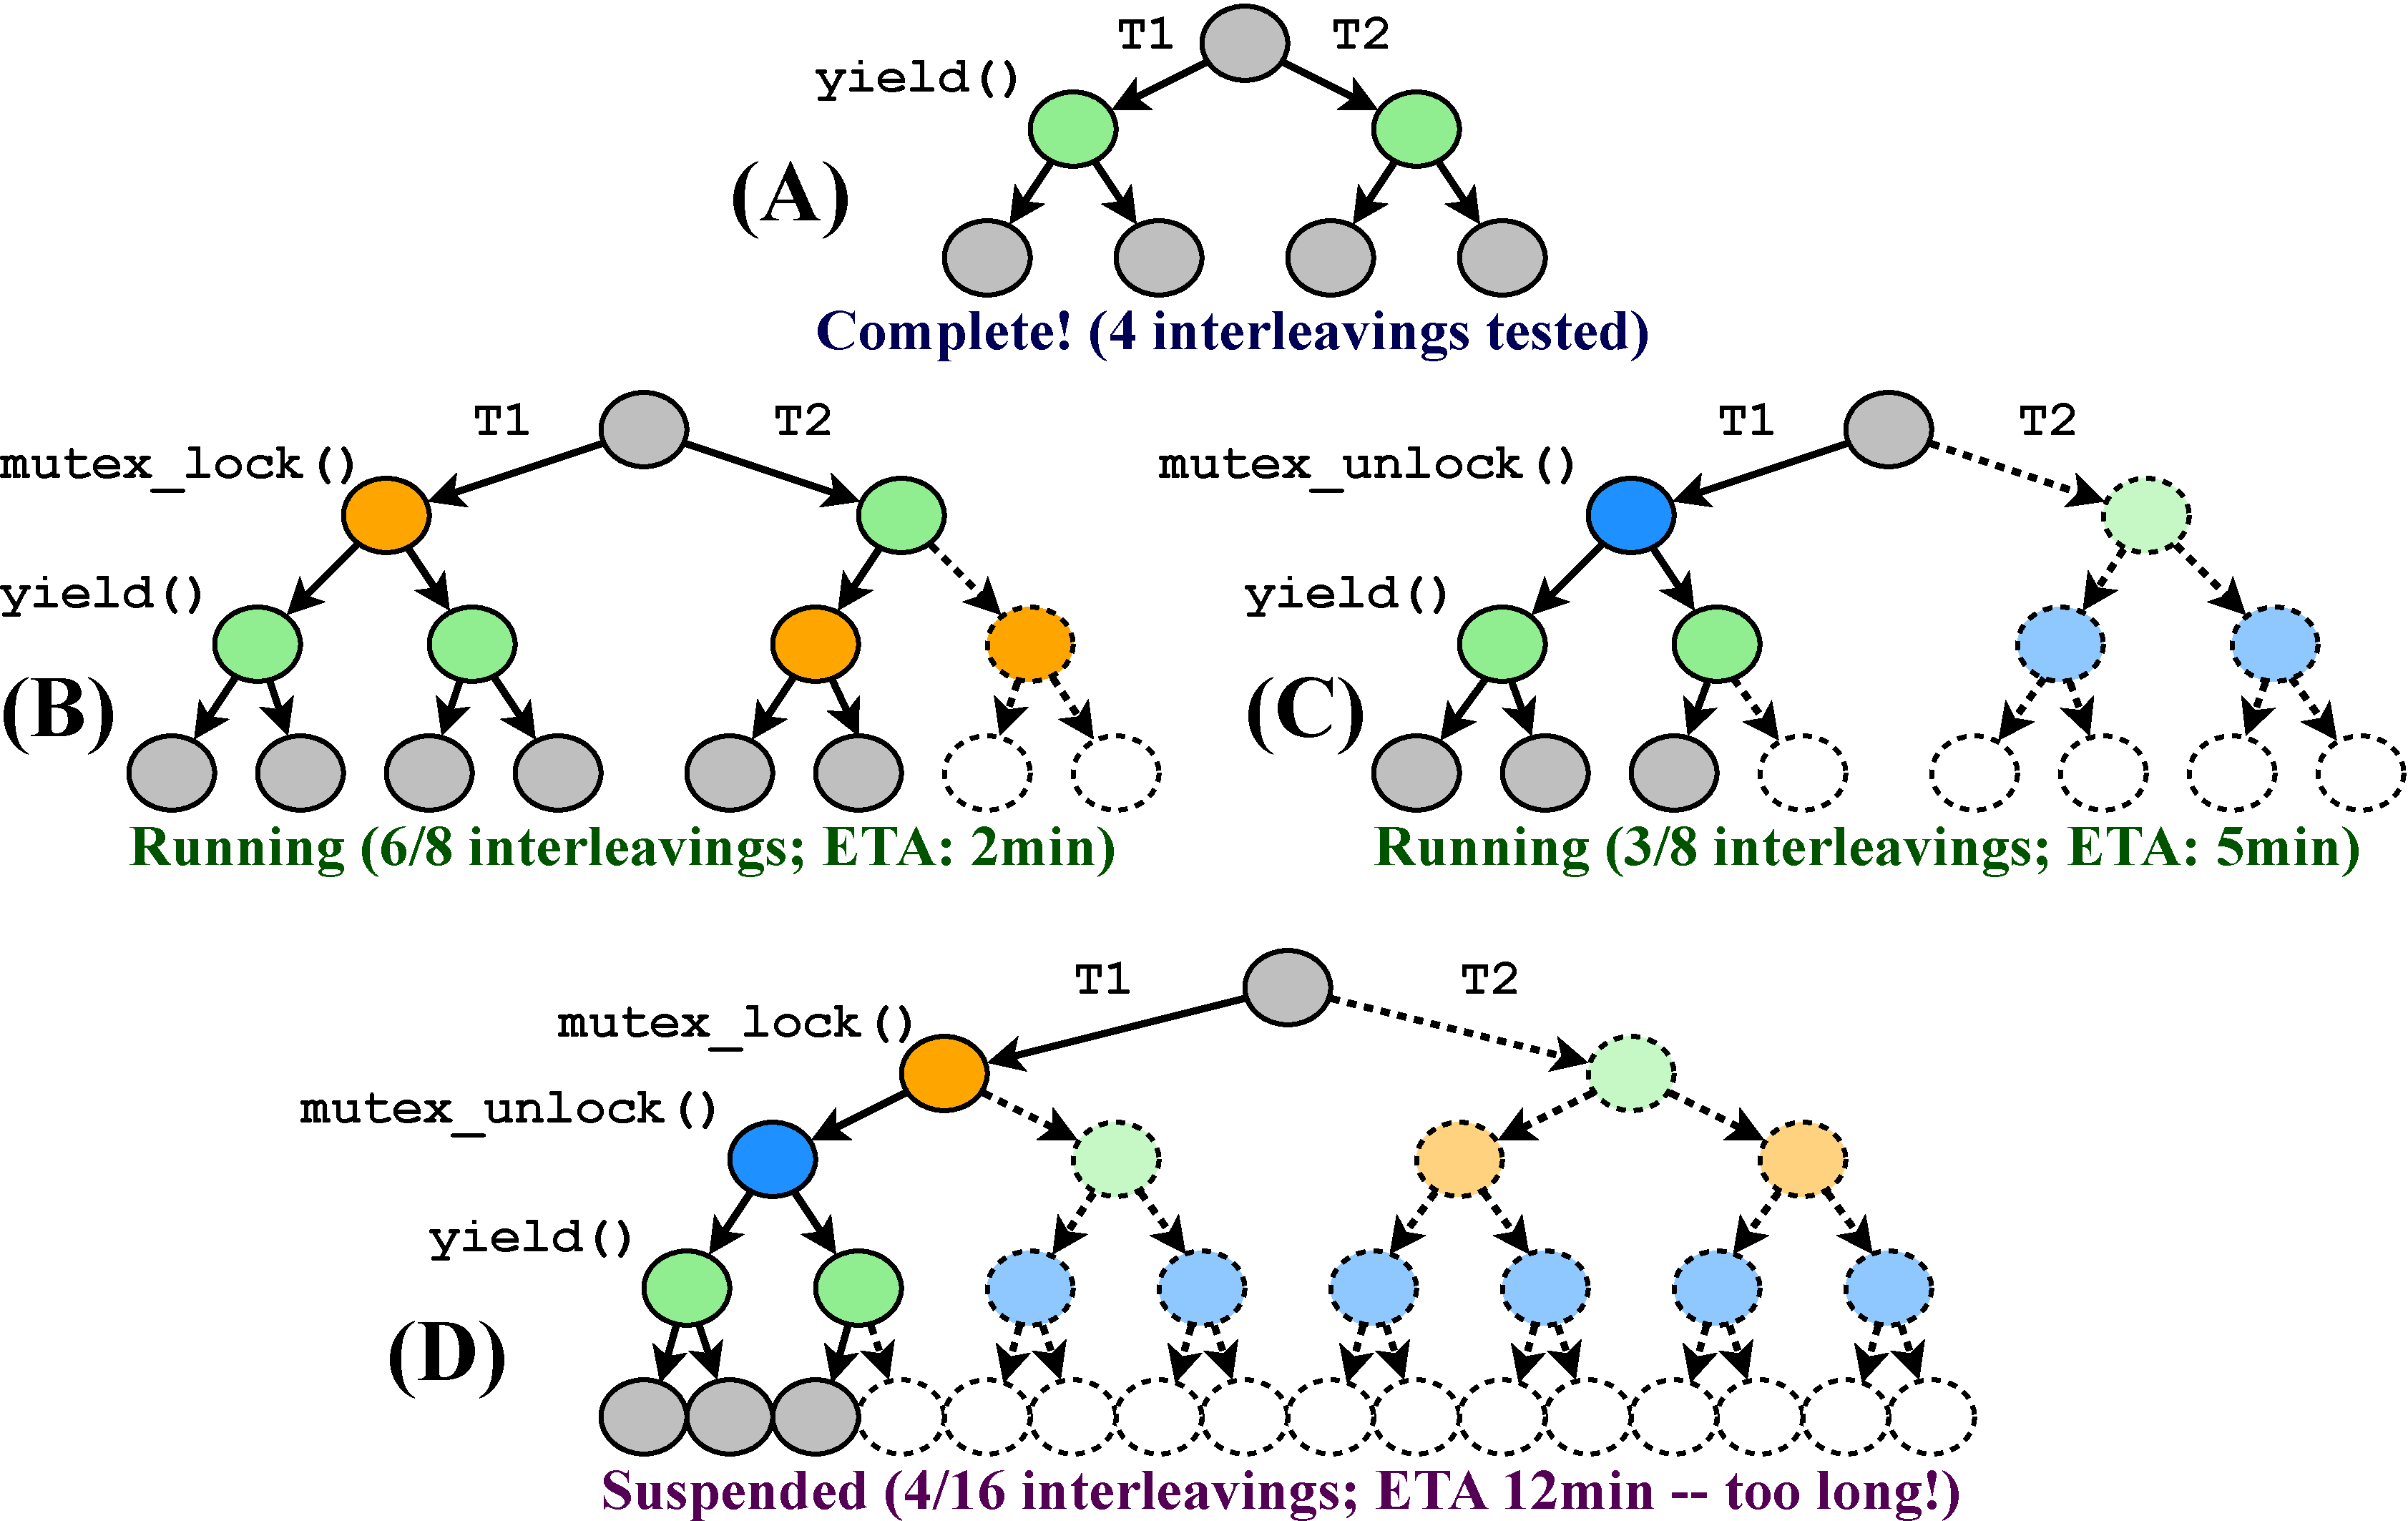
\includegraphics[width=0.48\textwidth]{trees-v2-squashed.pdf}
	\caption{Iterative Deepening example.
		The minimal state space (A) includes only voluntary thread switches, such as {\tt yield()}. %or {\tt cond\_wait()}.
		Multiple further tests can be run: preempting on calls to {\tt mutex\_lock} alone (B), {\tt mutex\_unlock} alone (C), or both together (D).
Each option increases the state space size unpredictably, so multiple state spaces should be tested in parallel.
Estimation techniques~\cite{estimation} inform which state spaces to prioritize.
}
	\label{fig:id}
\end{figure}

The checker defines the granularity of thread interleavings by the {\em preemption points} it uses to switch threads.
Most model checkers \cite{chess,dbug-ssv} choose synchronization/thread library API boundaries for these points;
in our example program, these would be lines 1, 4, and 7.
Figure~\ref{fig:id} shows several possible resulting state spaces.
The approach of prior work is to enable all preemption points simultaneously, i.e., to test only the state space denoted (D).

To mitigate the exponential explosion,
Dynamic Partial Order Reduction \cite{dpor} identifies equivalent execution sequences according to Mazurkiewicz trace theory \cite{mazurkiewicz},
and tests at least one execution from each equivalence class.
Intuitively, if two thread transitions between preemption points do not conflict on any shared resource access, reordering them produces an equivalent interleaving, i.e., the same program behaviour.
Nevertheless, state spaces are still exponentially-sized in the number of conflicting transitions.

This motivates {\em Iterative Deepening}, our new technique for heuristically adjusting the preemption points at runtime.
Rather than committing to one state space with every available preemption point enabled,
we will search among different {\em subsets} of the points.
%for example, ``preempt on all calls to {\tt mutex\_lock} but not on {\tt mutex\_unlock}''.
Hence, we will test all the state spaces shown in Figure~\ref{fig:id} in parallel,
and decide on-the-fly whether to pursue each test, or to defer it in favour of others.

\subsection{Data Race Detection}
\label{sec:overview-dr}

Data race analysis \cite{eraser} identifies pairs of unsynchronized memory accesses between threads.
Two instructions are said to race if
they both access the same memory address,
at least one is a write,
the threads do not hold the same lock,
and no synchronization enforces an order on the thread transitions \revision{(the {\em Happens-Before} relation)}.
Data races \revision{do not always lead to failures}, but represent suspicious violations of common locking discipline.
In Figure~\ref{fig:example}, lines 3 and 5 each race with 2 and 6, and line 6 races with 8.

\revision{
A data race analysis may be either {\em static} (inspecting source code) \cite{racerx} or {\em dynamic} (tracking individual accesses arising at run-time) \cite{tsan}.
This paper focuses exclusively on dynamic analysis,
so although our example refers to numbered source lines for ease of explanation,
in practice we are actually classifying the individual memory access events corresponding to those lines during execution.
}

%\revision{Among these, only the races involving lines 3 and 5 are relevant to the possible assertion failure;
%permuting the order of line 8 alone
%% relative to 2 and 6
%will not change the program's behaviour.}

Though state-of-the-art model checkers preempt only on synchronization events,
many serious concurrency bugs are caused by data races leading to corrupted shared state.
Figure~\ref{fig:example}'s buggy interleaving is possible only with {\em data-race preemption points}:
preempting just before an instruction identified as part of a data race.
None of the state spaces in Figure~\ref{fig:id} contain this interleaving,
as none of the mutex/yield preemptions split lines 2 and 6 across different transitions.

\revision{
	{\bf Variants of Happens-Before (HB).}
	Most prior work focuses on {\em Pure HB} \cite{lamport-clocks} as the order relation between accesses.
\cite{predictive-dr} and \cite{hybriddatarace} identify a problem with this approach:
it cannot identify access pairs separated by an unrelated lock operation which could race in an alternate interleaving,
as shown in the example program in Figure~\ref{fig:hb-example}(a).
We call such unreported access pairs {\em false negatives}.
\cite{hybriddatarace} introduces the {\em Limited HB} relation,
which will report such potential races
by considering only blocking operations like {\tt cond\_wait} to enforce the order.
However, consider the similar program in Figure~\ref{fig:hb-example}(b),
in which the access pair ceases to exist in the alternate interleaving.
Limited HB will report all potential races, avoiding false negatives \cite{tsan},
but at the cost of necessarily reporting some such {\em false positives}.
Finally, the {\em Causally-Precedes} relation \cite{predictive-dr} strikes a middle ground,
extending Pure HB to additionally report a subset of potential races while soundly avoiding false positives.

Stand-alone data-race analyses must avoid inundating the user with false alarms \cite{racerx}.
However, this work incorporates data-race analysis in an internal feedback loop,
using MC to automatically check each potential race
and reporting to the user only directly observed failures.
%Our convergence theorem requires identifying all potential data-races to provide total verification (\sect{\ref{sec:totalverif}})
%% TODO CAMREADY: cite our soundness proofs tech report in this paragraph as well
Hence, we employ Limited HB in this paper},
accepting some overhead from false positives for the sake of total verification (\sect{\ref{sec:totalverif}}).

\begin{figure}[t]
	\small
\begin{tabular}{c}
	\revision{
\begin{tabular}{rll}
	& \multicolumn{2}{c}{\texttt{int x = 0; bool y = false; mutex\_t mx;}} \\
	& {\bf Thread 1} & {\bf Thread 2} \\
	1 & \texttt{\hilight{brickred}{x++;}~// A1} & \\
	2 & \texttt{mutex\_lock(\&mx);} & \\
	3 & \texttt{mutex\_unlock(\&mx);} & \\
	4 & & \texttt{mutex\_lock(\&mx);} \\
	5 & & \texttt{mutex\_unlock(\&mx);} \\
	6 & & \texttt{\hilight{brickred}{x++;}~// A2} \\
\end{tabular}
}
\\
\revision{\normalsize (a) True potential data race.}
\\
\\
\revision{
\begin{tabular}{rll}
	%& \multicolumn{2}{c}{\texttt{int x = 0; bool y = false; mutex\_t mx;}} \\
	%& {\bf Thread 1} & {\bf Thread 2} \\
	1 & \texttt{\hilight{brickred}{x++;}~// B1} & \\
	2 & \texttt{mutex\_lock(\&mx);} & \\
	3 & \texttt{y = true;} & \\
	4 & \texttt{mutex\_unlock(\&mx);} & \\
	5 & & \texttt{mutex\_lock(\&mx);} \\
	6 & & \texttt{bool tmp = y;} \\
	7 & & \texttt{mutex\_unlock(\&mx);} \\
	8 & & \texttt{if (tmp) \hilight{brickred}{x++;}~// B2} \\
	%8 & & \texttt{if (tmp)} \\
	%9 & & \texttt{~~~~\hilight{brickred}{x++;}~// B2} \\
\end{tabular}
}
\\
\revision{\normalsize (b) No data race in any interleaving.}
\end{tabular}
\caption{\revision{Data-race analyses may be prone to either {\em false negatives} or {\em false positives}.
Applying Pure HB to program (a) will miss the potential race possible between A1/A2 in an alternate interleaving,
while using Limited HB on (b) will produce a false alarm on B1/B2.}}
\label{fig:hb-example}
\end{figure}

% Old explanation.
%Prior work \cite{hybriddatarace} distinguishes between {\em pure happens-before} \cite{lamport-clocks},
%in which accesses with a lock release/acquire in between are not considered concurrent,
%and {\em limited happens-before},
%in which only blocking operations like {\tt cond\_wait} or {\tt join} enforce the order.
%Compared to the former, the latter may report false positives, but avoids false negatives \cite{tsan},
%in which a potential racing access pair is not reported, even though it could lead to a bug.
%We use the limited happens-before analysis, accepting some overhead from false positives for the sake of total verification (\sect{\ref{sec:totalverif}}).

\subsection{Terminology}

For the rest of the paper, we will abbreviate {\em preemption point} (PP),
%For the remainder of the paper, we will abbreviate {\em preemption point} (PP),
{\em model checking} (MC),
{\em single-state-space model checking} (SSS-MC), % (i.e., the approach of prior work),
{\em Dynamic Partial Order Reduction} (DPOR), and {\em state space estimate} (ETA).

SSS-MC indicates the approach of prior tools:
the set of PPs is fixed in advance, and the tool commits to testing every interleaving available with those PPs.
%Reduction techniques are often used to skip equivalent interleavings \cite{dpor}, and search-ordering strategies
Many techniques can skip equivalent interleavings or order the search to uncover bugs faster \cite{dpor,demeter,chess-icb,gambit,smc-empirical-study},
but new PPs cannot be added, nor ineffective ones removed, by any dynamic analysis.

Although all data races are undefined behaviour in C and C++ \cite{boehm-memorymodels},
we distinguish between data-race {\em candidates} and data-race {\em bugs}.
% old explanation
%Because data-race analysis is prone to false-positives,
%we classify unprotected memory access pairs separately from bugs,
\revision{We refer to racing (or potentially-racing) memory access pairs as}~{\em data race candidates}.
Should a future interleaving, preempting during such accesses,
lead to \revision{an observable}~failure, then we report a {\em data-race bug}.
Otherwise, if the access pair can be reordered \revision{to be simultaneous}, but does not produce a failure under any interleaving, it is a {\em benign data race} (with respect to the test input).
If they cannot be reordered at all, due to some other communication \revision{such as in Figure~\ref{fig:hb-example}(b)}, it is a {\em false positive}.

We also identify the {\em minimal} and {\em maximal state space} for each test.
The {\em minimal state space} includes only thread switches arising from normal execution (Figure~\ref{fig:id}, A).
The {\em maximal state space} is the one tested by SSS-MC: all statically-available PPs are enabled (Figure~\ref{fig:id}, D).
%However, should new data-race PPs be added during a test, the new maximal state space will be the one including those as well.
%% don't say this ^ -- because when you add dr pps, they add in pairs and there would be multiple maximals, at least until they each get explored and subseuqnetly add a pp of the other of the pair.
